\section{Metodologia}

\subsection{Single Board Computer (SBC)}

Single Board Computer (SBC) é um computador onde todas os componentes necessários estão em uma mesma placa de circuito impresso. Esse tipo de dispositivo é muito utilizado para fins educacionais, para desenvolvimento de sistemas, datacenters (centros  de  processamento  de  dados) e clusters portáteis. Alguns exemplos são o \textit{OrangePI}, \textit{RockPI}, \textit{BeagleBone} e \textit{RaspberryPI}, sendo este um dos mais populares \cite{SBC_edu}.

Os SBCs possuem baixo custo, porém devido a escassez global de semicondutores aumentou o preço da maioria deles


Para este trabalho foi selecionado o SBC \textit{OrangePI} devido a custos. O preço sugerido para o \textit{RaspberryPI} é de 35 dólares 


\subsubsection{RaspberryPI}

A \textit{Raspberry Pi Foundation} foi fundada em 2008 sediada no Reino Unido com o objetivo de promover o avanço na educação no campo da computação. \cite{rasp}

\begin{figure}[!htbp]
  \caption{Raspberry Pi 3}
  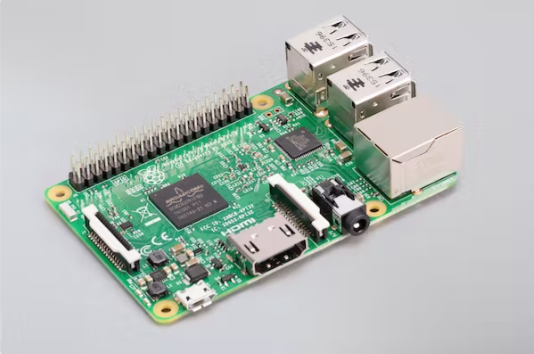
\includegraphics[scale=0.5]{images/rasp.png}
  \legend{Fonte: \citeauthor{rasp_prod}}
  \label{figura:rasp}
\end{figure}


\subsubsection{OrangePI}

Variante chinesa do RaspberryPI

\begin{figure}[!htbp]
  \caption{Orange Pi 3 LTS}
  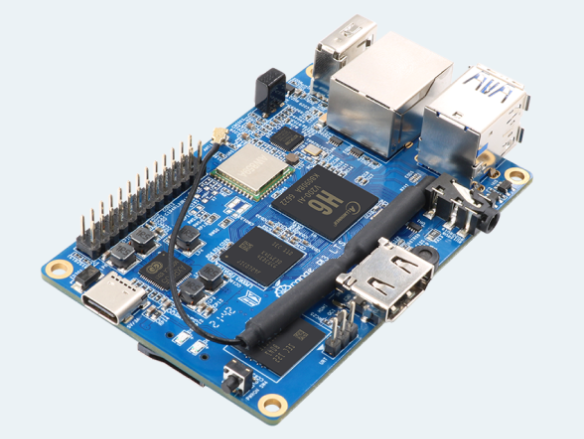
\includegraphics[scale=0.4]{images/orange.png}
  \legend{Fonte: \citeauthor{orangepi}}
  \label{figura:orange}
\end{figure}

